\chapter{Suy luận kiểu - Type inference}

Đối với bài toán Suy luận kiểu, trình dịch ngược không được cung cấp các thông tin về kiểu union như ở bài toán Kiểm tra kiểu mà phải dựa vào việc phân tích quá trình sử dụng dữ liệu của chương trình để xác định các union tồn tại trong chương trình. Việc giải quyết bài toán này gồm các bước sau:

\begin{itemize}
	\item Vì chưa có thông tin về các vùng nhớ có kiểu union trong chương trình, nên bước đầu tiên chỉ dừng lại ở việc xác định vùng nhớ mà thanh ghi trung gian đang mang tại mỗi thời điểm của chương trình.
	\item Dựa vào các câu lệnh có sử dụng những đối tượng dữ liệu truy xuất đến một phần của một vùng nhớ, xác định được vùng nhớ nào có kiểu là union cũng như các thành phần thuộc union đó.
\end{itemize}

Hai phần tiếp theo sẽ lần lượt trình bày các bước trên.

\section{Xác định vùng nhớ thanh ghi trung gian đang mang tại mỗi thời điểm của chương trình}

Ở ngôn ngữ assembly, các vùng nhớ được đại diện bởi địa chỉ của chúng, vì vậy việc xác định vùng nhớ thanh ghi trung gian đang mang thực chất là xác định giá trị của địa chỉ vùng nhớ đó. Để xác định được giá trị này, phương pháp phân tích Lan truyền hằng số - Constant propagation sẽ được áp dụng. Như đã giới thiệu ở phần \ref{sec:constantprop}, mục tiêu của Lan truyền hằng số là xác định giá trị của một biến tại một thời điểm của chương trình có phải là hằng số hay không và giá trị của hằng số đó là bao nhiêu. Điều này phù hợp với yêu cầu của bài toán.

Tuy nhiên, trong một kiến trúc máy, có những thanh ghi được dùng làm thanh ghi trung gian cho việc xử lý vùng nhớ và có những thanh ghi thì không được, tuỳ thuộc vào tính chất của thanh ghi mà hằng số cần lan truyền sẽ khác nhau. Trong đoạn mã \ref{list:accdptr}, ở câu lệnh số 2 biến \textit{a} (đại diện cho một thanh ghi trung gian ở ngôn ngữ assembly) đang được truyền vào giá trị vùng nhớ được một con trỏ trỏ tới. Trình dịch ngược không quan tâm đến việc giá trị vùng nhớ được trỏ tới là bao nhiêu, mà chỉ quan tâm đến việc địa chỉ của vùng nhớ này, tức giá trị của con trỏ, là gì để phân biệt được với những vùng nhớ khác. Như vậy, chỉ có biểu thức nằm trong dấu * mới cần tính toán giá trị xem có phải là hằng số không. Tiếp tục với ví dụ đó, biểu thức nằm trong dấu * lại là một biến khác, biến \textit{dptr} (đại diện cho một thanh ghi không được sử dụng làm thanh ghi trung gian ở ngôn ngữ assembly). Như vậy, để tìm ra được địa chỉ vùng nhớ được truyền vào biến \textit{a}, thì chương trình cần phải tính toán giá trị thật sự của biến \textit{dptr}. Hay nói cách khác, hằng số cần tìm đối với biến \textit{dptr} là giá trị của toàn bộ biểu thức nằm bên phải phép gán ở câu lệnh số 1.
\begin{lstlisting}[caption={Đoạn mã thể hiện hai loại thanh ghi},label={list:accdptr}]
dptr = OPTIONS; //1
a = *(dptr); //2
\end{lstlisting}

Như vậy, có thể kết luận:
\begin{itemize}
	\item Đối với những thanh ghi trung gian, trình dịch ngược chỉ quan tâm đến việc nó đang được load vào vùng nhớ nào, còn việc giá trị thực sự của thanh ghi này là gì thì không quan trọng. Vì vậy, với loại thanh ghi này, hằng số cần tìm ra là giá trị của địa chỉ vùng nhớ mà nó đang mang.
	\item Đối với những thanh ghi khác, chúng chỉ được xét đến khi xuất hiện trong biểu thức quy định giá trị địa chỉ vùng nhớ ở các câu lệnh gán vùng nhớ cho thanh ghi trung gian. Vì vậy, trình dịch ngược chỉ quan tâm đến giá trị thật sự của những thanh ghi này để tính toán giá trị của địa chỉ vùng nhớ đó. Như vậy, hằng số cần tìm của loại thanh ghi này là giá trị thực sự mà thanh ghi đó đang mang.
\end{itemize}

Vì tính chất trên, cần phải chỉnh sửa phân tích Lan truyền hằng số cho phù hợp với yêu cầu của bài toán. Tuỳ thuộc vào loại thanh ghi, mà biểu thức được lấy ra để tính hằng số sẽ khác nhau. Giải thuật Lan truyền hằng số đã có sửa đổi được trình bày ở hình \ref{fig:constantpropagationalgo2}. Phần có đường viền nhạt hơn là phần được thêm vào để phù hợp với yêu cầu bài toán.
\begin{figure}
	\centering
	\includegraphics[scale=0.70]{image/constantPropagationAlgo2}
	\caption{Giải thuật Constant propagation đã được chỉnh sửa để áp dụng vào trình dịch ngược}
	\label{fig:constantpropagationalgo2}
\end{figure}

Ngoài ra, để tính toán được giá trị thực sự của một biến, cần phải có một hàm chức năng nhận vào một biểu thức và trả về được giá trị của biểu thức đó. Có rất nhiều cách để hiện thực chức năng này, sau một quá trình xem xét, visitor sẽ được sử dụng cho việc tính toán giá trị của biểu thức. Visitor \cite{dessignpattern} là một pattern design trong các chương trình lập trình hướng đối tượng, nó được dùng để tách một thuật toán ra khỏi cấu trúc dữ liệu mà thuật toán đó sử dụng. Lợi ích đạt được là người lập trình có thể thêm những chức năng mới cho cấu trúc dữ liệu đó mà không cần thay đổi kiến trúc của nó. Điều này phù hợp với nhu cầu hạn chế tối đa việc thay đổi các mã có sẵn khi hiện thực các giải pháp của luận văn trên một trình dịch ngược nào đó.\\

Để hiện thực pattern design này, cần tạo ra một class visitor và viết hàm visit cho các loại biểu thức. Các hàm visit này chính là nơi tính toán và trả về giá trị của biểu thức. Các biểu thức ở mức độ assembly thường được viết rất đơn giản, bao gồm các dạng chính sau:
\begin{itemize}
	\item Một hằng số.
	\item Một biến được khai báo trước.
	\item Một thanh ghi, giá trị của thanh ghi có thể được khai báo ở các câu lệnh trước đó.
	\item Một biểu thức có hai vế, các vế của biểu thức có thể là một biến, một thanh ghi hoặc một hằng số.
\end{itemize}
Vì vậy, trong class visitor này chỉ cần có một số hàm visit cho các loại biểu thức sau đây:

\begin{itemize}
	\item \textit{Const}: Là biểu thức hằng số. Hàm visit này chỉ đơn giản trả về giá trị hằng số nếu đây là một hằng số nguyên.
	\item \textit{Binary}: Là biểu thức có 2 vế. Hàm visit sẽ visit từng vế của biểu thức, và nếu cả hai vế đều là hằng số, thì sẽ thực hiện phép tính cộng trừ nhân chia hai hằng số đó để ra được kết quả cuối cùng.
	\item \textit{RefExp}: Loại biểu thức này chứa một biểu thức khác, kèm theo câu lệnh khai báo biểu thức đó. Trong giới hạn nhu cầu của bài toán, chỉ những RefExp chứa biểu thức là một biến hoặc một thanh ghi được tính toán tiếp, còn những loại biểu thức khác sẽ mặc định trả về giá trị là bottom. Giá trị của tên biến hoặc thanh ghi này sẽ được tìm kiếm trong danh sách lưu trữ dữ liệu.
	\item \textit{TypedExp}: Loại biểu thức để ép kiểu một biểu thức nào đó thành kiểu mong muốn. Với trường hợp này, giá trị trả về của biểu thức ép kiểu chính là giá trị của biểu thức con bên trong.
\end{itemize}

Với phương pháp phân tích này, vấn đề vế phải của phép gán thanh ghi là những biểu thức phức tạp có hai toán hạng đã được giải quyết. Ngoài ra, phân tích này còn nhận biết được các biểu thức có giá trị giống nhau mặc dù hình thức bên ngoài khác nhau. Xem ví dụ các câu lệnh ở đoạn mã \ref{list:listdiffassignacc}. Câu lệnh gán số 1 và số 2 thực chất đều gán cho \textit{ACC} giá trị vùng nhớ có địa chỉ quy định bởi biến \textit{OPTIONS}. Nếu thực hiện phân tích Reaching definitions ở giải pháp trước, trình dịch ngược sẽ không thể biết được điều này. Tuy nhiên, ở giai đoạn này, vì trình dịch ngược sẽ tính toán được ở cả hai câu lệnh, \textit{ACC} đều mang giá trị của vùng nhớ có địa chỉ là \textbf{38}. Và ở những bước tiếp theo, trình dịch ngược sẽ đối chiếu giá trị \textbf{38} với bảng lưu trữ dữ liệu và biết được biến \textit{OPTIONS} đại diện cho giá trị đó.

\begin{lstlisting}[caption={Một số câu lệnh gán cho ACC có giá trị vế phải bằng nhau},label={list:listdiffassignacc}]
#DEFINE OPTIONS #38
#DEFINE CLAMP #37
...
MOV ACC, OPTIONS
MOV ACC, CLAMP+1
\end{lstlisting}

Một ưu điểm nữa của phân tích Lan truyền hằng số là đối với các câu lệnh phi, câu lệnh thể hiện một biến có thể có nhiều giá trị khác nhau, thì giải thuật sẽ tính toán những giá trị đó xem chúng có phải là hằng số và những hằng số đó có bằng nhau hay không. Nếu bằng nhau, có thể kết luận rằng biến này vẫn là hằng số cho dù luồng đi của chương trình như thế nào. Điều này sẽ giúp tăng độ chính xác hơn so với các giải thuật phân tích trước đó, vốn xử lý trường hợp này bằng cách bỏ qua và mặc định xem như biến này không phải hằng số.

Như vậy, phân tích Lan truyền hằng số đã giải quyết được những trường hợp mà 2 phân tích được giới thiệu trước đó là Reaching definitions kết hợp phần mở rộng và Lan truyền kiểu không giải quyết được. Sau khi xác định được các vùng nhớ mà thanh ghi trung gian đang mang thông qua địa chỉ của nó, bước tiếp theo để giải quyết bài toán này là tìm kiếm những thành phần của union đại diện cho vùng nhớ đó.
\section{Xác định thành phần của các union đại diện cho vùng nhớ}

Với bài toán Suy luận kiểu, do chưa có những thông tin về kiểu union và các thành phần của union, nên ở bước này trình dịch ngược phải phân tích và tìm ra những thông tin đó dựa vào đoạn mã chương trình. Ý tưởng để hiện thực việc tìm kiếm này như sau:
\begin{itemize}
	\item Chạy vòng lặp qua các câu lệnh của chương trình, khi gặp một câu lệnh sử dụng một biến được khai báo là đại diện cho một phần của thanh ghi trung gian thì kiểm tra thanh ghi trung gian đang mang giá trị của vùng nhớ có địa chỉ là bao nhiêu. 
	\item Thực hiện các bước kiểm tra xem việc sử dụng union này có hợp lý hay không. Nếu hợp lý, trình dịch ngược sẽ ghi nhận tên biến này là tên thành phần thuộc union đại diện cho vùng nhớ mà thanh ghi trung gian đang mang. 
\end{itemize}
Như đã phân tích ở phần trước, một vùng nhớ được đại diện bởi con số thể hiện địa chỉ của nó, nếu dùng cấu trúc UnionDefine đã được giới thiệu ở chương trước thì không có thành phần nào thể hiện con số này. Như vậy, cần phải mở rộng cấu trúc UnionDefine để lưu trữ được địa chỉ của vùng nhớ mang kiểu union. Cấu trúc UnionDefine dành cho mã 8051 đã mở rộng được thể hiện ở đoạn mã \ref{list:listnewuniondefine} với thành phần byteVarValue được thêm mới.
\begin{lstlisting}[caption={Đoạn mã mới của class UnionDefine},label={list:listnewuniondefine},language=c++]
class UnionDefine{
	public:
		char* byteVar;
		map<int, char*>* bitVar;
		int byteVarValue;
};
\end{lstlisting}
Như vậy, mục tiêu của bước này là xây dựng nên các thực thể UnionDefine hoàn chỉnh, bao gồm trường thể hiện địa chỉ vùng nhớ mang kiểu union và tên các thành phần thuộc union đó. Quá trình này được thể hiện ở hình \ref{fig:stepunionmaking}.
\begin{figure}[h]
	\centering
	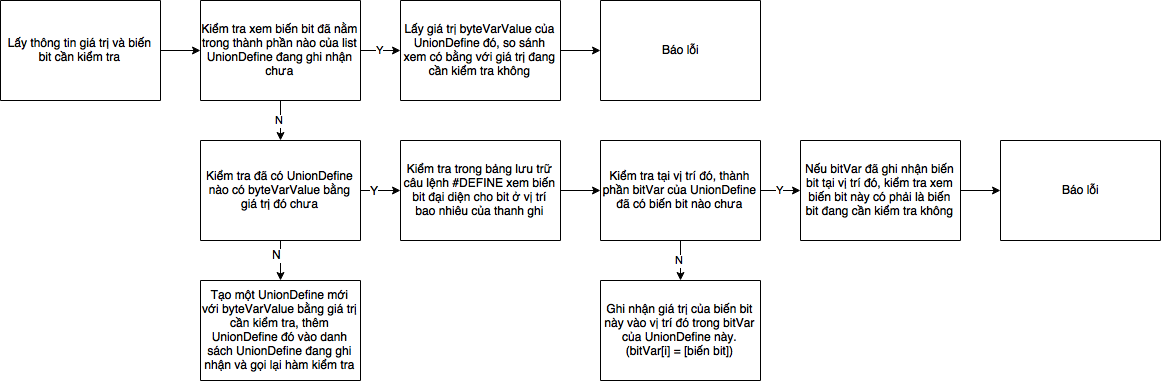
\includegraphics[width=\linewidth]{image/stepUnionMaking}
	\caption{Các bước kiểm tra và ghi nhận dữ liệu vào danh sách UnionDefine}
	\label{fig:stepunionmaking}
\end{figure}

Sau quá trình trên, trình dịch ngược đã xác định được các thành phần của union đại diện cho một vùng nhớ được xác định bằng địa chỉ. Tuy nhiên, từ giá trị của địa chỉ vùng nhớ, cần phải suy ra được tên thật sự của union bằng cách tìm kiếm tên biến được khai báo mang giá trị đó. Ví dụ như ở đoạn mã \ref{list:varval}, biến \textit{OPTIONS} khai báo có giá trị là hằng số \textbf{38H}. Nếu sau một quá trình phân tích, trình dịch ngược tìm được một union đại diện cho vùng nhớ có địa chỉ \textbf{38H}, thì cần phải chuyển giá trị \textbf{38H} này về lại \textit{OPTIONS} để ra được tên của union. 
\begin{lstlisting}[caption={Đoạn mã khai báo một biến có giá trị là hằng số},label={list:varval}]
#DEFINE OPTIONS, #38H
\end{lstlisting}
Quá trình chuyển đổi này khác đơn giản do ở giai đoạn parser đã có lưu thông tin về cặp biến - giá trị, nên chương trình chỉ cần dò tìm trong bảng này để lấy ra được tên biến tương ứng với giá trị của địa chỉ vùng nhớ. Trong trường hợp không có tên biến nào được khai báo có giá trị trên, trình dịch ngược sẽ tự động sinh ra một tên biến mới có định dạng: \textbf{\textit{LOCATION\_[giá trị]}}, ví dụ: \textit{LOCATION\_38}.

Như vậy, với danh sách các thực thể UnionDefine tìm thấy được thông qua các bước trình bày ở trên, bài toán Suy luận kiểu union đã được giải quyết.